\section*{Raccolta dati}
La raccolta dati è basata su due fonti principali: YouTube e OurWorldInData della Oxford University.

\subsection*{Youtube API}
I video in tendenza su Youtube variano ogni 15 minuti circa (fonte: \url{https://support.google.com/youtube/answer/7239739?hl=it}). Tuttavia questo non significa che cambino effettivamente i contenuti presenti, infatti solitamente si assiste solo a qualche video che scompare dalle tendenze o viceversa nuovi video che appaiono. Va specificato inoltre che il numero assoluto di video in tendenza è di circa 200, con qualche calo durante la notte più rilevante.

Le API di Youtube ci hanno permesso di raccogliere i dati necessari riguardanti i video in tendenza, con delle limitazioni sul numero di richieste gratuite che si potessero fare mediante il Google Developer.
\\
Sono state affrontate due sessioni di \textit{scraping} con metodi leggermente differenti:
\begin{enumerate}
	\item dal 23 dicembre 2019 al 5 gennaio 2020 (richieste ogni 30 minuti)
	\item dal 18 marzo 2020 al 6 maggio 2020 (richieste ogni 6 ore)
\end{enumerate}
Abbiamo deciso di raccogliere dati delle tendenze dei seguenti paesi:

Italia, USA, Regno Unito, India, Germania, Canada, Francia, Corea del sud, Russia, Giappone, Brasile, Messico\\

\subsection*{Prima sessione}
L'idea che ha guidato la fase iniziale del progetto era quella di comprendere come l'algoritmo delle tendenze di Youtube sceglie i video, utilizzando caratteristiche come visualizzazioni, likes, dislikes e commenti. La raccolta dati ha seguito il seguente algoritmo, messo in pratica dallo script \textit{scraper\_csv.py}:\\
\\
\begin{algorithm}[H]
	\KwData{country - insieme dei paesi prescelti; videos - insieme di video scaricati da un determinato paese}
	\nl \For{every 30 minutes} {
	\nl \ForEach{country}
	{
		\nl videos = APIrequest(max(50 video), country)\\
		\nl \While {tendency videos are finished}
		{
			\nl videos += APIrequest(max(50 video), country) \\
		}
		\nl videos\_fix = arrangeData(videos)\\ 
		\nl saveToCsv(videos\_fix) \\
		\nl videos = $\emptyset$
	}
	}
	\caption{Scraper csv}
\end{algorithm}

%Alternativa per scrivere l'algoritmo
%\begin{enumerate}
%	\item Per ogni paese prescelto
%	\item API request sulle tendenze del momento $\rightarrow$ download di page da 50 video [formato json]
%	\item ripeti 2. finchè scarica tutti i video
%	\item copio le informazioni formattate in formato csv (vedi dopo) 
%	\item ripeti da 2. per ogni paese
%	\item attendi 30 minuti (scheduler)
%	\item ripeti da 1.
%\end{enumerate}
\underline{Nota}: per ogni richiesta API è possibile scaricare un massimo di 50 video, inoltre ogni paese ha un numero di video differente (solitamente 150-200).

I dati vengono salvati in formato \textit{csv} secondo il seguente schema:
\begin{table}[H]
	\centering
	\begin{tabular}{l|l}
		\textbf{Attributo} & \textbf{Descrizione} \\
		\hline
		\textbf{timestamp} & data, ora e minuto della nostra rilevazione \\\hline
		\textbf{video\_id} & identificativo unico del video\\\hline
		\textbf{title} & nome del video per esteso\\\hline
		\textbf{publishedAt} & data di pubblicazione\\\hline
		\textbf{channelId} & identificativo unico del canale che ha pubblicato il video\\\hline
		\textbf{channelTitle} & nome del canale per esteso\\\hline
		\textbf{categoryId} & identificativo unico della categoria\\\hline
		\textbf{trending\_date} & data in cui il video è in tendenza\\\hline
		\textbf{tags} & stringa contenente i tag usati, separati dal carattere "|"\\\hline
		\textbf{view\_count} & numero di visualizzazioni\\\hline
		\textbf{likes} & numero di like (mi piace)\\\hline
		\textbf{dislikes} & numero di dislike (non mi piace)\\\hline
		\textbf{comment\_count} & numero di commenti sotto il video\\\hline
		\textbf{thumbnail\_link} & url all'immagine di copertina del video\\\hline
		\textbf{comments\_disabled} & booleano che dichiara se i commenti sono disabilitati\\\hline
		\textbf{ratings\_disabled} & booleano che dichiara se i like/dislike sono disabilitati\\\hline
		\textbf{description} & descrizione del video\\
		\hline
	\end{tabular}
	\caption{schema degli attributi dei dati csv}
\end{table}

I dati così raccolti sono salvati in una cartella che può essere definita al momento dell'avvio dello script mediante l'argomento \textit{-o}.

\subsection*{Seconda sessione}

Lo scoppio della pandemia da Covid-19 ci ha permesso di cambiare approccio e domande di ricerca, cercando di valutare come la pandemia abbia influenzato Youtube. Con l'esperienza della presa dati precedente abbiamo cambiato metodo di raccolta, preferendo immagazzinare i dati direttamente, attraverso una pipeline, in un database MongoDB.

Inoltre abbiamo effettuato cambiamenti all'algoritmo di scraping, preferendo effettuare le richieste API ogni sei ore, per un totale di quattro rilevazioni al giorno, invece che ogni 30 minuti come prevedeva precedentemente lo schema.

A scopo didattico abbiamo deciso di implementare una piccola pipeline Kafka in cui dividiamo la fase di raccolta dati (\textit{scraper\_producer.py}) e la fase di immagazzinamento (\textit{scraper\_consumer.py}). 

\begin{figure}[H]
	\centering
	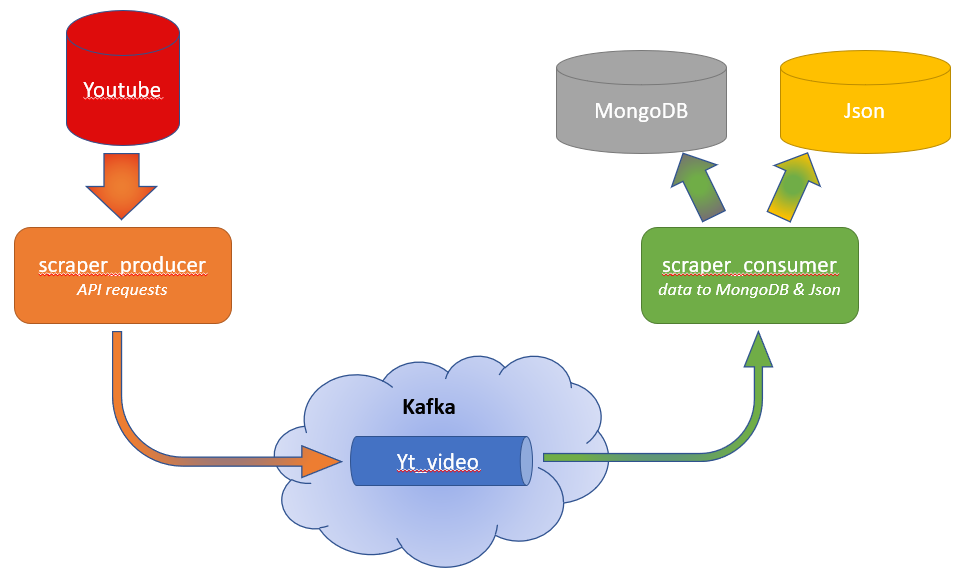
\includegraphics[width=0.8\linewidth]{pics/pipeline.png}
	\caption{pipeline di raccolta dati - seconda sessione}
\end{figure}

Di seguito si può vedere nel dettaglio il procedimento dei due algoritmi:

\begin{algorithm}[H]
	\KwData{country - insieme dei paesi prescelti; videos - insieme di video scaricati da un determinato paese; KafkaProducer(data, channel) - sends data to channel kafka}
	\nl \For{every 6 hours} {
		\nl \ForEach{country}
		{
			\nl videos = APIrequest(max(50 video), country)\\
			\nl KafkaProducer(videos, yt\_video) \\ 
			\nl \While {tendency videos are finished}
			{
				\nl videos = APIrequest(max(50 video), country) \\
				\nl KafkaProducer(videos, yt\_video) \\
			}
		}
	}
	\caption{scraper producer}
\end{algorithm}

\begin{algorithm}[H]
	\KwData{KafkaConsumer(channel) - receives data from channel kafka}
	\nl \While{loop} {
		\nl \If{KafkaConsumer(yt\_video) $\ne \emptyset$}
		{
			\nl videos = KafkaConsumer(yt\_video)\\
			\nl videos\_fix = arrangeData(videos)\\ 
			\nl saveToJson(videos\_fix)\\
			\nl saveToMongoDB(videos\_fix)
		}
	}
	\caption{scraper consumer}
\end{algorithm}
I dati così raccolti sono stati salvati in formato json, è possibile definire la cartella di output in cui vengono salvati i file mediante il comando \textit{-o}. 

\underline{Nota}: I dati sono stati salvati in json per avere una maggior facilità nel caricare i dati su MongoDB. Il caricamento è stato eseguito mediante lo script \textit{json\_to\_mongo.py}

Lo schema logico dei documenti json è sostanzialmente invariato rispetto a quello della prima sessione, eccetto per due variazioni:
\begin{itemize}
	\item \textbf{tags} immagazzinati come array di stringhe.
	
	Ad esempio:
	
	tags: ["covid-19", "quarantena"]
	
	\item informazioni relative ai likes, dislikes, view\_count e comment\_count come documenti innestati nella chiave \textbf{statistics}.
	
	Ad esempio:
	
	statistics: \{view\_count: 14235,
				likes: 513,
				dislikes: 34,
				comment\_count: 254
				\}
\end{itemize}
\subsection*{Dati Covid-19}

I dati relativi alla pandemia, come il numero di contagi totali o giornalieri, sono stati ottenuti dal sito \href{https://ourworldindata.org/coronavirus-testing}{OurWorldInData} dell'università di Oxford. Successivamente abbiamo eseguito una prima manipolazione per ottenere i dati che interessavano i paesi e le date che abbiamo considerato. I risultati vengono visualizzati in un file \textit{csv}:
\begin{table}[H]
	\centering
	\begin{tabular}{l|l}
		\textbf{Attributo} & \textbf{Descrizione} \\
		\hline
		\textbf{iso\_code} & codice unico riferito al paese \\\hline
		\textbf{location} & nome esteso del paese\\\hline
		\textbf{date} & data della rilevazione\\\hline
		\textbf{total\_cases} & numero totale dei casi\\\hline
		\textbf{new\_cases} & nuovi casi registrati in quella giornata.\\\hline

	\end{tabular}
	\caption{Schema degli attributi dei dati sul Covid-19.}
\end{table}

